%-----------------------------------------------------------------
%	DATA BACKGROUND
%	!TEX root = ./../main.tex
%-----------------------------------------------------------------
\subsection{Sea surface temperature}\label{ssec:sst}

\subsubsection{Description of the database}\label{ssec:hadisst-intro}
There are several sea surface temperature (SST) databases, with different time-steps (e.g., daily, weekly, monthly, and so on), domains (i.e., global or specific regions), and data resolutions; each used for different analyses of climatological nature~\cite{o:sst-comparison, Rayner2003}.

The Met Office~\cite{o:met-office} Hadley Centre's sea ice and sea surface temperature database, HadISST1~\cite{o:hadisst1}, is a unique combination of monthly globally complete fields of SST and sea ice concentration on a latitude-longitude grid from 1871. In \Cref{fig:sst-raster-map} we can see a sample from the data set to illustrate the grid structure.

Although there is a revised HadISST.2 database~\cite{o:hadisst2}, we use the HadISST1 database, as it is the one used in \citeauthor{Corral2010}'s, \citeauthor{Webster2005}'s and several other authors's climate analyses.

The main reason to do so, however, is that HadISST.2 contains more ocean grid boxes and introduces a different method to calculate the monthly temperatures, making it quite incompatible with HadISST1 (as opposed to the revised HURDAT2 database, which is just an improved version of the old database, without introducing changes in the methodology of analysis or in the structure of the data).

\begin{figure}[H]
	\centering
	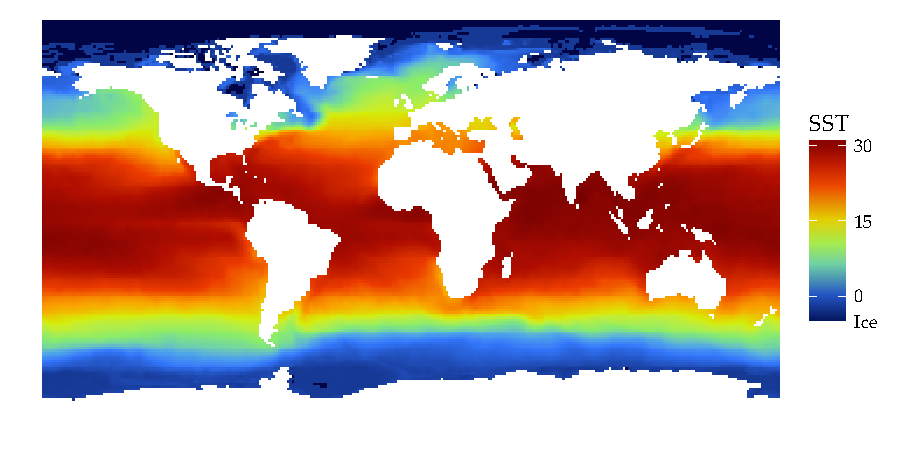
\includegraphics[width=\textwidth]{images/sst-raster-map}
	\caption{Global SST (in \si{\celsius}) map from December 2015}
	\label{fig:sst-raster-map}
\end{figure}

%-----------------------------------------------------------------
\subsubsection{Data structure}
The format of the HadISST1 database is documented at~\cite{o:hadisst1-format}. The data are available in netCDF format, which is constructed using raster data.

A raster brick consists of a matrix of cells (or pixels) organised into a grid where each cell contains a value representing information, such as temperature in our case. Each matrix can also be comprised of layers (as illustrated in \Cref{fig:raster}); in the HadISST1 database, each matrix layer represents a different month.
\begin{figure}[H]
	\centering
	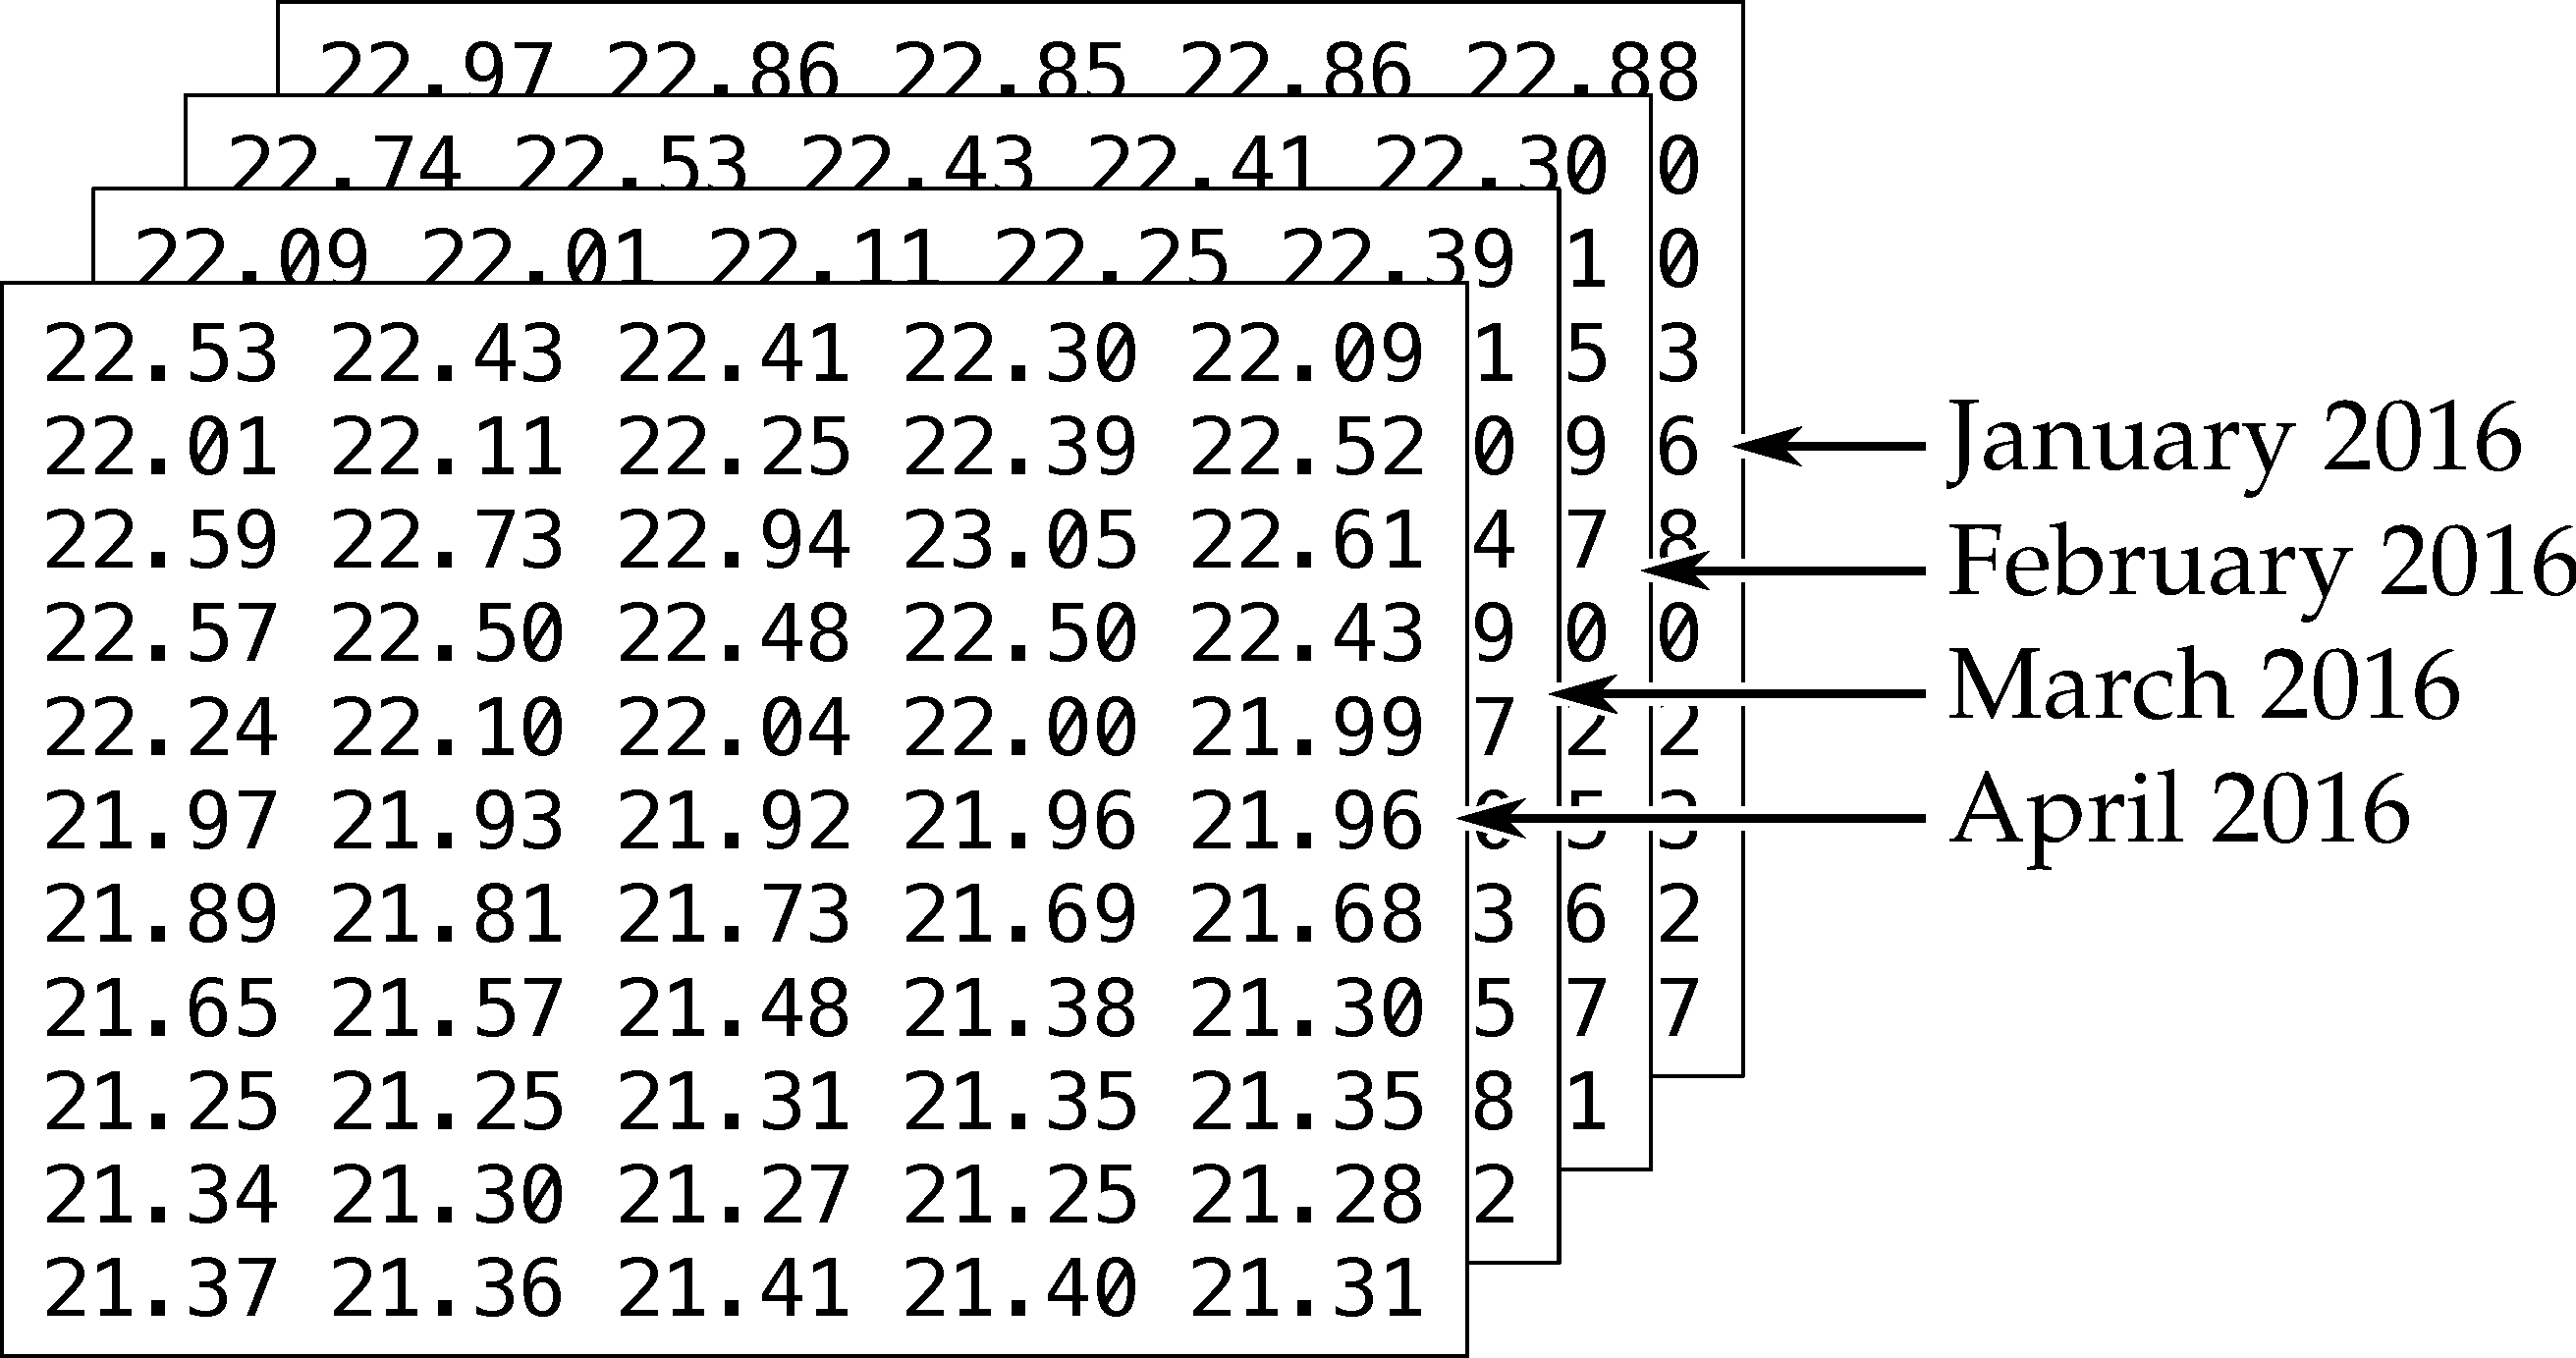
\includegraphics[width=0.7\textwidth]{images/raster}
	\caption{Simple diagram of the internal structure of a raster brick}
	\label{fig:raster}
\end{figure}

The data set used can be downloaded from \url{http://www.metoffice.gov.uk/hadobs/hadisst/data/HadISST_sst.nc.gz}.

\bigskip
% \todo[inline]{paragraph about the SST class}
In \Cref{hd:sst-head} one can see the structure of the result from the SST classification of the years into low-SST and high-SST to illustrate the variables we use, as well as the data type of the SST data. Note that the classification is unique to each of the basins.
\begin{table}[H]
	\centering
	\ttfamily
	\begin{tabular}{r r r r}
		\toprule
		\toprule
		year & sst & sst.norm & sst.class \\
		<date> &   <dbl>   &  <dbl> &    <chr> \\
		\midrule
		1966-01-01 & 27.47 & 0.9979934 &  low \\
		1967-01-01 & 27.19 & 0.9879054 &  low \\
		1968-01-01 & 27.34 & 0.9933687 &  low \\
		1969-01-01 & 27.75 & 1.0083072 & high \\
		1970-01-01 & 27.36 & 0.9940200 &  low \\
		1971-01-01 & 27.04 & 0.9825272 &  low \\
		\bottomrule
	\end{tabular}
	\caption{Excerpt of the results from the SST analysis for the North Atlantic basin}
	\label{hd:sst-head}
\end{table}
